\section{Structure of Codebase}
The codebase is twofold, where one part is for object detection and the other part is for movement and interaction with the motors.
\todo{figure out whether the python part also does the calibration or not}
The object detection part, which is run on a Raspberry Pi, is written in Python 3{.}7, and the movement processing is handled by the NXT and is written i C, version C90 with GNU-extensions.


\subsection{Object Detection}
The codebase is seperated into modules with the intent of creating a system where each module can be exchanged based on different contexts and further development.
The following modules exist:
\begin{itemize}
	\item Object Localization Algorithm
	\item Output / Communication
	\item Input / Webcam
\end{itemize}

These are all utilized by a controller class, called \texttt{FlatController}, that ties the solution together, which has the signature shown in snippet~\ref{lst:FlatControllerInit}.
\begin{lstlisting}[language=Python,label={lst:FlatControllerInit},caption={Initialization method of the \texttt{FlatController} class}]
def __init__(self,
	algorithm: Callable[[np.ndarray], Vector],
	video_controller: webcam.VideoController,
	output_devices: Union[OutputDevice, List[OutputDevice], None] = None,
	) -> None:
	"""
	Initializes the controller
	:param output_devices: The device to send data to
	:param algorithm: The algorithm to use for image processing
	:param video_controller: The controller handling the input video
	"""
\end{lstlisting}

The order of the parameters doesn't correspond to the order of relevance, but rather is a requirement as two of the parameters have default arguments.
This method takes, as the signature shows, a function, \texttt{algorithm} with an array as input and a vector as output.
This array is the array of pixels in a given frame.
The intent of this algorithm is to take a given frame, and localize the target within the frame.


\todo{implement the video output debug to actually be what i've written below}
The \texttt{output\_devices} parameter is a class that handles transmitting the location data to the NXT, but this can be overwritten to use a video feed as output as well, with the intent of debugging. 
This argument can either be a singular \texttt{OutputDevice} or multiple, which is relevant when the user both wants to debug but also transmit the information to the NXT device.


\todo{maybe change the capture\_type to also be either a class or a function, so we follow the same paradigm of coding all the way through}
Lastly the \texttt{capture\_type} parameter handles from which device the video feed should come from.
By default this should be a camera feed, but it might be relevant to use a specific video file in some contexts, for instance when doing tests.


The controller is initialized in the \texttt{main.py} file, which is the entry point when running the program, often from the commandline. The relevant arguments are shown in snippet~\ref{lst:MainHelp}.
\begin{lstlisting}[label={lst:MainHelp},caption={The help message of the commandline interface}]
$ python3 main.py --help
usage: main.py [-h] [-a [name]] [-d]

Run the object detection part of the F.L.A.T system

optional arguments:
-h, --help            show this help message and exit
-a [name], --algorithm [name]
Choose which algorithm to run [GOTURN, YOLO, ZONE_AVG, OBJ_FILL]. default='obj_fill'
-d, --debug           Whether to run in debug mode. whether to show video feed
\end{lstlisting}
\todo{make sure these are still up to date when finishing the project, also image, bellow it isn't as Teknight created a new algorithm- but yeah}
Figure~\ref{fig:pythonClasses} shows the dependencies of each of the actual packages, and how each module is split up, into multiple packages or files.

\begin{figure}[H]
	\centering
	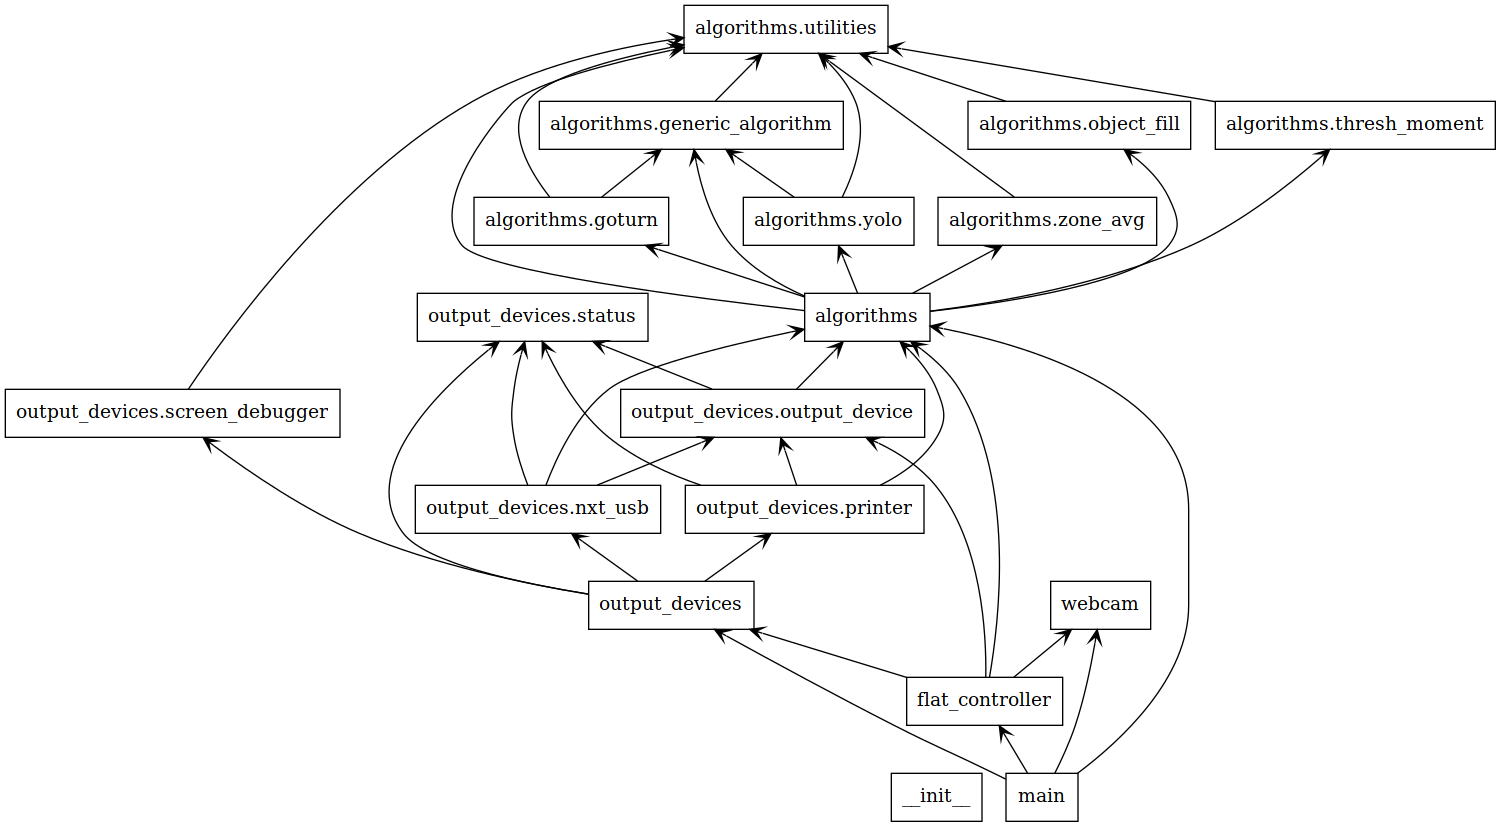
\includegraphics[width=\textwidth]{5.Solution/images/python_packages.png}
	\caption{The dependencies of the packages of the project{.} Image generated with pyreverse\cite{pyreverse}}
	\label{fig:pythonClasses}
\end{figure}


The project also contains functions for calibration, as seen on figure~\ref{fig:pythonClasses}, which will be covered in section~\ref{sec:calibration}.


\subsection{Movement}
The codebase is not in the same way seperated into modules, in a direct way, due to the design of the language. However the solution is divided into multiple file with distinct responsibilities.

\begin{itemize}
	\item \texttt{tasks}
	\item \texttt{usb}
	\item \texttt{display}
	\item \texttt{movement}
	\item \texttt{calibration}
\end{itemize}

the \texttt{tasks.c} can be seen as the primary file of the project, which creates all the tasks that the scheduling system enforces.
The code in snippet~\ref{lst:taskDecl} piece of code declares the tasks, but the specific aspects of each tasks, will be covered more indepth in section~\ref{sec:scheduling}
\begin{lstlisting}[language={c},label={lst:taskDecl},caption={Declaration of tasks, counters and events}]
/* OSEK declarations */
DeclareTask(ReceiveData);
DeclareTask(UpdateDisplay);
DeclareTask(ToggleLaser);
DeclareTask(MoveMotors);

DeclareCounter(SysTimerCnt);

DeclareEvent(MoveMotorsOnEvent);
DeclareEvent(MoveMotorsOffEvent);
DeclareEvent(LaserOnEvent);
DeclareEvent(LaserOffEvent);

DeclareResource(USB_Rx);
\end{lstlisting}
\todo{update above}
Rec


This file is not manually run, so less can be set about the overall principles of how it is run, as this is handled by the NXT-OSEK operating system, however the dependencies still seem relevant, which are detailed in figure~\ref{fig:CClasses}
\todo{insert picture here when we are done - i don't want to spend time creating one}


Each of these files and modules will be explained in-depth throughout this chapter, and explain value of each.

\
